\documentclass[useAMS,usenatbib]{mn2e}
%%%%% AUTHORS - PLACE YOUR OWN MACROS HERE %%%%%%%%%%%%%%%%%%
\usepackage{graphicx}
\usepackage{epstopdf}
\epstopdfsetup{outdir=./}
\usepackage{color}
%\usepackage{floatpag}
\usepackage[pdftex, hidelinks]{hyperref}
\newcommand {\aplt} {\ {\raise-.5ex\hbox{$\buildrel<\over\sim$}}\ }
%\setlength\parindent{0pt}
%%%%%%%%%%%%%%%%%%%%%%%%%%%%%%%%%%%%%%%%%%%%%%%%


\title[The SGP at 145\,MHz with PAPER]{Measurements of the Southern Galactic Plane at 145\,MHz with PAPER: evidence of synchrotron self-absorption?}

\author[S. A. Kohn et al.]{S.~A. Kohn,$^{1}$\thanks{E-mail: saulkohn@sas.upenn.edu} J.~E. Aguirre,$^{1}$ W. Saunders,$^{1}$
A.~Parsons,$^{2,3}$
\newauthor et al.$^4$\\
$^{1}$ Department of Physics and Astronomy, University of Pennsylvania, Philadelphia, PA 19104\\
$^{2}$ Astronomy Dept., U. California, Berkeley CA\\
$^{3}$ Radio Astronomy Lab., U. California, Berkeley CA\\
$^{4}$ a lot of other places\\
}
\begin{document}
\date{}

\pubyear{2015}
\maketitle
\begin{abstract}
Present astrophysical understanding of high-mass stars allows for predictions of their formation rates.  High-mass stars explode in supernovae, which leave behind Supernova Remnants (SNRs) that serve as records of the stars; however the $\sim$300 observed SNRs is far fewer than the $>1000$ predicted.  This gap could implicate the understanding of high-mass stars if confirmed. 
Meanwhile, there is presently a dearth of low-frequency radio measurements ($\nu\aplt$200\,MHz) of sources in the Southern Galactic Plane (SGP).
This study reports on a search for SNRs as well as measurements of sources in the SGP using low-frequency radio maps produced at 145\,MHz by Precision Array for Probing the Epoch of Reionization (PAPER).
{\color{red} VERY BRIEF SUMMARY OF FINDINGS.}
{\color{blue} CAN WE ARGUE FOR GOOD POINTS OF LOW-RES?}
%Mathematical predictions {\color{red}[CITE!!]} of the number of observable SNRs based on known limitations showed that the SNR Defect may be made up by a complete survey.  This shows that the SNR Defect is likely due to selection effects: difficulties in detecting SNRs given their location and size, and not due to a fundamental misunderstanding in star formation rates.
\end{abstract}

\begin{keywords}
ISM: molecular clouds -- stars: formation
\end{keywords}

\section{Introduction}

The Southern Galactic Plane (SGP) has been measured at various radio frequencies, including the Molonglo Galactic Plane Surveys \citep[MGPS-1 and 2;][]{Green.99,Murphy.07} and the Molonglo Observatory Synthesis Telescope SNR Catalog \citep[MOSTSNRCAT;][]{Whiteoak.96} at 843\,MHz and the Southern Galactic Plane Survey \citep[SGPS;][]{Haverkorn.06} at 1.4\,GHz. Synthetic catalogs of SNRs at 1\,GHz \citep{DAGreen.14} and H{\sc ii} regions at 2.7\,GHz \citep{Paladini.03} also cover the SGP, and infrared measurements were made by, e.g., the Midcourse Space Experiment \citep[MSX;][operating at 8.28--21.3\,$\mu$m (36.23--14.08\,THz)]{Egan.03}. 

However, there is a dearth of measurements of the SGP at very low radio frequencies ($\nu\aplt$200\,MHz). In this work, we present {\color{red}low-resolution} measurements of the SGP at 145\,MHz.  Currently the only counterpart to such measurements were presented in the 7C(G) survey of the Northern Galactic Plane \citep{Vessey.98} which was conducted at 151\,MHz. 

{\color{red} WHY IS LOW FREQ AWESOME?}

\subsection{Supernova Remnants}
The major classification difference between high-mass ($M > 8M_{\odot}$ ) and low-mass ($M < 8 M_\odot$) stars is the end of their life, for which the latter explode in supernovae (SNe), which is precipitated by accumulated inert iron in the core \citep{Arnett.73}.  
The subsequent collapse of the core creates the supernova explosion, which ejects the entirety of the star’s outer layers, forming a supernova remnant (SNR).  The SNR consists of the expanding supernova shock wave, the ejected outer material of the star, and any dust or gas it picks up while expanding.  
The remnant slowly expands until its density becomes near that of the surrounding interstellar medium (ISM) making it effectively indistinguishable, and ending its existence as an SNR.  


The SNR shock releases high-velocity particles, including a barrage of electrons that produce non-thermal emissions; these relativistic electrons are accelerated and spiraled by the magnetic fields of the SNR and produce synchrotron radiation as a result making SNRs easily-detectable radio sources \citep[e.g.][]{Burbidge.56,Stupar_cat.11}. 
SNRs are relatively short-lived ($\sim10^5$ yr), which means that they can serve as a record of recent star formation rates of high-mass stars -- by counting SNRs, one can hope chart recent star formation.
Measuring the star formation rates through iron abundance allows for a reasonable prediction of the number of galactic SNRs; however, these predictions imply that there should be far more SNRs than currently detected \citep[e.g.][]{Brogan.06}.  

To date, 294 SNRs have been catalogued \citep{DAGreen.14} despite the prediction based on the Galactic star formation rate that $\sim10^3$ galactic SNRs exist \citep{Li.91,Pavlovic.13}.  
Additionally, \cite{Brogan.06} made estimates based on known limitations of radio surveys in order to predict the number of SNRs that are observable at all.
Their study yielded a result of 460 observable SNRs; this is still less than half of the observed value. 
This “SNR Defect” has thus far been attributed to selection effects including: 
\begin{itemize}
\item[(i)] SNRs occur in dusty regions, where the dust may absorb and/or deflect SNR emissions;
\item[(ii)] since the vast majority of stars are located along the galactic plane, so are most SNRs, increasing potential source confusion \citep[e.g.][]{Gao_v.11,Gao_vi.11};
\item[(iii)] due to the inverse square law of observed luminosity,% doubling the distance to an object reduces its apparent brightness by one-fourth. 
the light from SNRs located 50,000 ly away, for example, is diminished by a factor of $\sim$300  \citep{Green.91};
\item[(iv)] superpositioning along the Earth’s line of sight, by which nearby, young  and inherently dense SNRs block or severely inhibit the entire field of view behind them, making surveys of the SNR population more difficult. 
\end{itemize}

{\color{red}[NOW WE NEED TO SAY SOMETHING ABOUT HOW LOW-FREQ CAN HELP WITH THIS]}
Radio observations should be able to resolve some of these selection effects. Dust neither attenuates nor scatters at radio frequencies. Young SNRs, which are compact and have close-to-blackbody emission spectra are more easily detected by optical surveys, whereas older SNRs, which are more diffuse and emit mostly at lower frequencies, are better detected with radio surveys.

\subsection{H{\sc ii} regions and misidentification}
While observing at radio frequencies mitigates most of the confusion when observing the Galactic plane, H{\sc ii} regions pose a more significant problem.  H{\sc ii} regions, opposed to SNRs, thermally emit from heating caused by nearby OB stars. % Recent discoveries {\color{red}[CITE!!!]} that some SNRs were actually galactic H{\sc ii} regions have increased the push for surveys to better differentiate them {\color{red}[for example (survey, rather than single one below)?]}.  
For example, SNR G166.2+2.5 was discovered to be an H{\sc ii} region heated by O7.5V star BD+41 1144 \citep{Foster.06}.  


Some larger SNRs, such as W28 (18h01m22.7s -23$^{\circ}$17'20") and W30 (18h03m -21$^{\circ}$30'), have positioned within them H{\sc ii} regions and other sources of thermal emissions, which increase the likelihood of misidentification \citep{Andrews.85}. \cite{Brogan.06} showed that the small likelihood of actual proximity notwithstanding, the apparent proximity interferes with detection of SNRs.  As a result, much has been invested in finding a method to mitigate the selection effects.\\

%Radio surveys have typically been used to observe shell-like SNRs %and are successful 
%because of the emission spectra and morphology of those SNRs \citep{Bandiera.01}.  {\color{red}[NEEDS MORE EXPLANATION -- this is a conference talk, we %should cite a resultant publication]}

% \cite{Stupar_cat.11} searched for H$\alpha$ emission coming from known radio-detected SNRs in order to better resolve detailed structure.  %X-ray surveys have also been successful in observing SNRs, but usually require supplemental information due to known limitations {\color{red}[for example...?]} \citep{Bandiera.01}.


This work presents measurements of sources in the SGP using the Precision Array for Probing the Epoch of Reionization (PAPER), a low-frequency radio telescope that observes at a central frequency of 145\,MHz. The paper is laid out as follows. In section~\ref{sec:obs} we discuss the acquisition and reduction of PAPER's measurements of the SGP. Section~\ref{sec:res} presents our map of the SGP, with detections of SNRs, H{\sc ii} regions and extragalactic sources cross-matched with the many of the catalogs listed above. We investigate those sources which do not match with any of the catalogs. In Section~\ref{sec:disc} we {\color{red} DISCUSS THINGS}. We summarize and conclude our study in Section~\ref{sec:conc}, with an eye towards future imaging surveys with PAPER and its successor, the Hydrogen Epoch of Reionization Array (HERA).

\begin{figure}
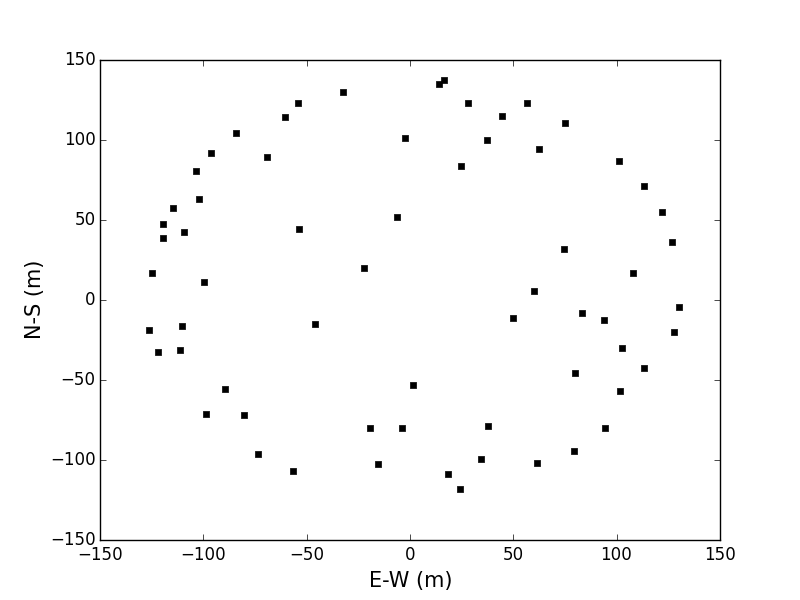
\includegraphics[width=\columnwidth]{psa64imageconfig.png}
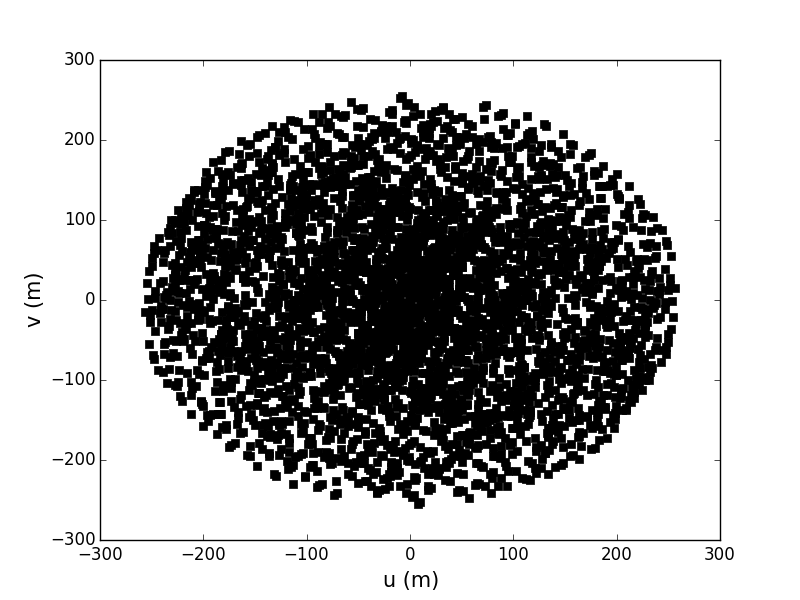
\includegraphics[width=\columnwidth]{psa64uvcoverage.png}
\caption{\textit{Above}: The PAPER-64 single-polarization configuration that took the measurements we report on in this paper. The antennae were arranged in a pseudo-random scatter in order to optimize uv-coverage. \textit{Below}: The resultant instantaneous uv-coverage, masking the very-short baselines ($\aplt 10 \lambda$). Maximum voxel occupancy is $\sim10$.}
\label{fig:config}
\end{figure}

\section{Observations}
\label{sec:obs}

The Precision Array for Probing the Epoch of Reionization (PAPER) is an experiment designed to set the strongest limits on, and possibly detect, the 21\,cm signal of neutral hydrogen at redshifts $z \geq 7.5$. It is operated in the Karoo, South Africa (-30:43:17.5 N, 21:25:41.9 E). To be able to set the strong limits it has to date \citep{Parsons.14, Jacobs.14, Ali.15, Moore.15}, it requires a highly redundant configuration to maximise its sensitivity to a few discrete uvw voxels \citep{Parsons.12}. However, in July and September 2011 the array was briefly reconfigured into an imaging array in order to do image-based analysis of the low-frequency radio sky \citep[e.g.][]{Jacobs.11, Stefan.13}. The imaging configuration and its instantaneous uv coverage is shown in Figure~\ref{fig:config}. Antennae were arranged in a pseudo-random scatter within a 300\,m-diameter circle, granting resolutions between 15' and 25' across the band.
Drift-scan visibilities were measured every 10.7 s, and divided into datasets about 10 minutes in length. PAPER antennae cannot point. However, within each dataset we are able to phase to the median zenith post-data-acquisition, and image accordingly. In this work we present single-polarization measurements made overnight July 4--5th 2011.

\section{Data reduction}
\label{sec:reduc}

All calibration was performed using the Astronomical Interferometry in PYthon ({\sc{aipy}}) package\footnote{\url{https://github.com/AaronParsons/aipy}}. Cross-talk removal was performed, and RFI removal masked channels that persistently showed large deviations from smooth-spectrum foregrounds (mainly due to known communications satellite bands). This removed approximately 30\% of the available bandwidth, and most removal occurred at the high and low ends of the band -- PAPER's excellent RFI environment allows most of the contiguous band to be used. Visibilities of bright extragalactic radio sources (e.g. Virgo A, Cygnus A) and the Sun were modelled and removed from the data. 


The data sets were self-calibrated to obtain complex gain solutions for each antenna, and then imaged, averaging over the whole 100\,MHz-wide band. Each image (dataset) was w-projected with a uv matrix resolution of 0.4 and a w-plane resolution of 0.1, and CLEANed \citep{Clark.80} to one part in $10^4$. These images were then used as `facets' and gridded to a HEALPix \citep{Gorski.05, Gorski.11} sphere with pixel size of 1 arcmin, subsequently convolved with a 2D Gaussian (FWHM=6 arcmins) to reduce pixelization effects. Finally, a cut in Galactic coordinates was made to extract the SGP ($25<l<230$, $-7.5<b<7.5$).


\subsection{Point-source calibration}
We were able to check the calibration described in Section~\ref{sec:reduc} against the extragalactic Molonglo Reference Catalogue \citep[MRC;][]{Large.81} sources measured by PAPER that are reported in \cite{Jacobs.11}. This comparison is shown in Figure~\ref{fig:PScal}, which exhibits a linear relation of

\begin{equation}
S^{145\,\rm{MHz}}_{\rm{Jacobs\,et\,al.}} = (0.9\pm0.2) S^{145\,\rm{MHz}}_{\rm{This\,work}} + (7\pm3)
\label{eq:PScal}
\end{equation}

This relation is within $2.5\sigma$ of direct proportionality alone, and taking into account the corrections to the \cite{Jacobs.11} flux scale, presented in \cite{Jacobs.13}, the margin closes to a direct proportionality.

\begin{figure}
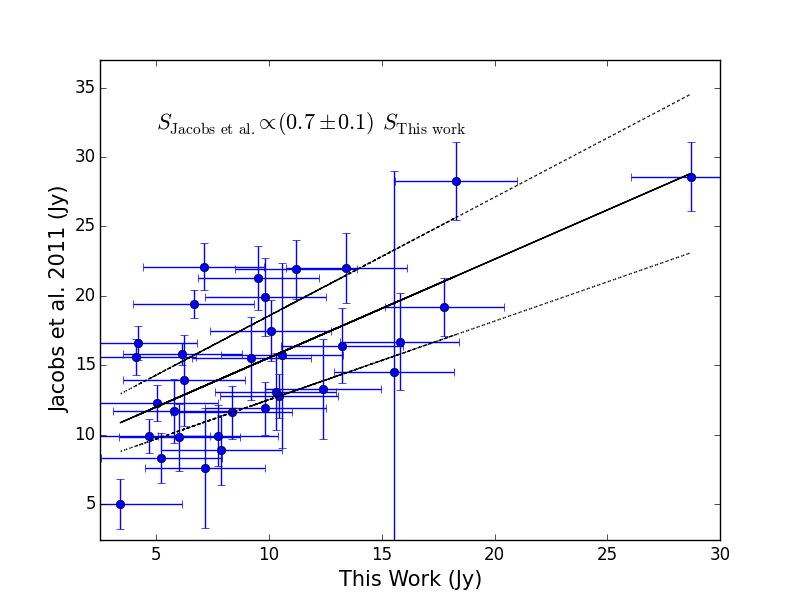
\includegraphics[width=\columnwidth]{us_and_danny_cal.png}
\caption{A comparison of the fluxes of extragalactic MRC sources measured by \protect\cite{Jacobs.11} at 145\,MHz, compared to our own. The measurements are consistent to within 1$\sigma$. The offset from direct proportionality is accounted for by corrections in \protect\cite[][see Section 3 of their paper]{Jacobs.13}.  A line of best fit is shown (solid line) along with $\pm1\sigma$ on the best fit parameters (shaded region).}
\label{fig:PScal}
\end{figure}

\section{Results}
\label{sec:res}

Our map of the SGP is shown in Figure~{\color{red}[NUMBER]... DETAILS}.

Source identification and extraction was performed using PyBDSM\footnote{\url{http://www.lofar.org/wiki/doku.php?id=public:user software:pybdsm}}, which identified all sources $\geq3\sigma$ above their local background, accounting for possible sidelobe confusion \citep{PyBDSM.15}. To each detected source we fit a two-dimensional, 20' FWHM Gaussian to approximate the PAPER beam \citep{Parsons.10} in order to extract the source flux. 

We detected $393$ individual sources, the properties of which are shown in Table~{\color{red}[NUMBER]... DETAILS}. In order to identify each detected source, we checked if any known sources were within the 20' PAPER beam at that position in the Galactic radio catalogues described in the introduction: MGPS, MOSTSNRCAT, the \cite{DAGreen.14} SNR catalogue and the \cite{Paladini.03} H{\sc ii} region catalogue. We also matched to the MRC sources detected in \cite{Jacobs.11}, a few of which (35) overlapped with our SGP cut. For the detected sources that were not within 20' of any objects in these catalogues (53), we queried the SIMBAD astronomical database \citep{Wegner.00} for any other SNRs,  H{\sc ii} regions, OB stars or undetected radio sources within the semi-major axis of the source.



\subsection{Comparison of Green SNR Fluxes with PAPER}

PAPER is not able to reconstruct flux on scales greater than $\sim3$
degrees due to missing baselines.  There is also the problem of source
confusion.  Basically, we have to look at the map to convince
ourselves that matches make sense; See Figure~{\color{red}[NUMBER]}.


{\color{red} The gold standard sources for source fluxes.}
For XXX Green sources which are relatively compact
and isolated, and with well-determined previous radio continuum
measurements, we construct the spectral index with PAPER and previous
measurements.  (Many are measured at 843\,MHz, etc ...; need to
reconsult literature to find original measurements.  Green presents a
synthetic point at 1\,GHz, and a spectral index.)


We also consider the classes of 1) Green SNRs with no previous or very
uncertain radio continuum detection (are there any?) ... do we see
them?  2) Green SNRs that are radio detected and smaller than $\sim3$
degrees, but PAPER does not detect.

Category 1: interesting, we provide the first flux.  Category 2:
synchrotron self-absorption??  Need to look at the expected flux at
150\,MHz relative to detection threshold.  

\subsection{Detection of {H\sc{ii}} regions at low frequencies}
We detect 13 {H\sc{ii}} regions that are listed in \cite{Paladini.03} at positions that do not appear in any other surveys we position-matched to. This is surprising, given that the expected emission mechanism, bremsstrahlung radiation, should be negligible at these frequencies...

\begin{table*}
\caption{Measured properties of {H\sc{ii}} regions}
\begin{tabular}{llllllll}
\hline
Name &  $\alpha$   &  $\delta$  &  PAPER Maj   &  Paladini Maj &  S$_{145}$  &  S$_{2700}$\\
 & J2000  &  J2000  &  arcmin  &  arcmin  &  Jy  &  Jy\\
\hline
000.3-00.5  &  266.83303  &  -29.185684  &  10.0 $\pm$ 1.0  &  3.0 $\pm$ 2.0  &  1.999 $\pm$ 2.341  &  2.5 $\pm$ 0.7 \\
006.0-01.3  &  271.06547  &  -24.443156  &  30.0 $\pm$ 6.0  &  9.0 $\pm$ 2.0  &  14.002 $\pm$ 2.512  &  44.9 $\pm$ 4.5 \\
006.0+00.1  &  269.75844  &  -23.693369  &  17.0 $\pm$ 2.0 &  7.0 $\pm$ 1.0  &  4.764 $\pm$ 2.702  &  38.2 $\pm$ 1.9 \\
006.1-00.1  &  270.08439  &  -23.671484  &  49.0 $\pm$ 6.0 &  6.0 $\pm$ 2.0  &  35.407 $\pm$ 2.09  &  18.0 $\pm$ 1.8 \\
006.3+02.0  &  268.13537  &  -22.548133  &  20.0 $\pm$ 3.0 &  7.0 $\pm$ 2.0  &  8.623 $\pm$ 2.672  &  1.2 $\pm$ 0.7 \\
006.6-00.3  &  270.34451  &  -23.396542  &  21.0 $\pm$ 0.0  & 7.0 $\pm$ 2.0  &  35.773 $\pm$ 2.932  &  54.0 $\pm$ 5.4 \\
006.6-00.1  &  270.26962  &  -23.259306  &  17.0 $\pm$ 1.0  & 2.0 $\pm$ 2.0  &  11.227 $\pm$ 2.727  &  11.1 $\pm$ 2.7 \\
007.0-01.1  &  271.53982  &  -23.228174  &  32.0 $\pm$ 11.0  & 3.0 $\pm$ 2.0  &  10.003 $\pm$ 2.378  &  0.3 $\pm$ 0.1 \\
007.0-00.3  &  270.95456  &  -23.058232  &  32.0 $\pm$ 11.0  & 5.0 $\pm$ 2.0  &  8.009 $\pm$ 2.497  &  13.0 $\pm$ 4.2 \\
007.5+00.7  &  270.01042  &  -21.80791  &  51.0 $\pm$ 14.0  & 2.0 $\pm$ 7.0  &  31.962 $\pm$ 1.612  &  5.1 $\pm$ 0.5 \\
011.9+02.2  &  270.86104  &  -17.556856  &  20.0 $\pm$ 5.0 &  0.0 $\pm$ 1.0  &  5.876 $\pm$ 2.691  &  1.0 $\pm$ 0.3 \\
015.0-00.7  &  275.14558  &  -16.205096  &  22.0 $\pm$ 3.0  & 6.0 $\pm$ 2.0  &  11.991 $\pm$ 2.701  &  489.0 $\pm$ 75.3 \\
017.0+00.8  &  274.65543  &  -13.772783  &  24.0 $\pm$ 4.0  & 16.0 $\pm$ 1.0  &  14.317 $\pm$ 2.577  &  107.0 $\pm$ 10.7 \\
021.0+02.0  &  275.5934  &  -9.6672018  &  24.0 $\pm$ 7.0  & 2.0 $\pm$ 1.0  &  6.024 $\pm$ 2.655  &  3.8 $\pm$ 1.7 \\
030.1+01.4  &  280.28398  &  -1.9022821  &  28.0 $\pm$ 7.0  & 1.0 $\pm$ 0.0  &  10.456 $\pm$ 2.505  &  1.1 $\pm$ 0.1 \\
034.1+00.5  &  282.91848  &  1.285108  &  56.0 $\pm$ 9.0  & 1.0 $\pm$ 0.0  &  34.367 $\pm$ 1.889  &  0.7 $\pm$ 0.1 \\
035.5-00.8  &  284.58448  &  1.6469897  &  36.0 $\pm$ 8.0  & 14.0 $\pm$ 8.0  &  14.604 $\pm$ 2.362  &  9.0 $\pm$ 2.7 \\
037.0-00.2  &  284.64053  &  3.7048426  &  40.0 $\pm$ 10.0  & 14.0 $\pm$ 7.0  &  17.735 $\pm$ 2.178  &  2.3 $\pm$ 1.2 \\
243.2+00.4  &  118.14421  &  -26.419824  &  18.0 $\pm$ 4.0  & 8.0 $\pm$ 11.0  &  5.248 $\pm$ 2.699  &  14.7 $\pm$ 2.1 \\
353.2+00.7  &  261.28827  &  -34.278429  &  22.0 $\pm$ 4.0  & 11.0 $\pm$ 2.0  &  7.158 $\pm$ 2.71  &  228.7 $\pm$ 46.0 \\
\hline
\end{tabular}
\label{tab:hii}
\end{table*}




\section{Discussion}
\label{sec:disc}

\begin{itemize}
\item SNR defect
\item We see HII regions?!
\end{itemize}

\section{Conclusions}
\label{sec:conc}

\begin{itemize}
\item Summarize findings
\item Brag about being the first low-freq measurements
\item Maybe brag about the maybe benefits of low-res measurements
\item Throw-out to polarized sky survey (Nunhokee et al. in prep.) and a future polarized galactic plane survey (Aguirre et al. in prep?).
\item Throw out to imaging capabilities of HERA\footnote{\url{www.reionization.org}}.
\end{itemize}

%\clearpage
\section*{Acknowledgements}
We thank SKA-SA for their efforts in ensuring the smooth running of PAPER. PAPER is supported through the NSF-AST program (awards 0804508, 1129258, and 1125558), the Mt. Cuba Astronomical Association, and by significant efforts by staff at NRAO. This research has made use of the SIMBAD database, operated at CDS, Strasbourg, France.


\appendix
\section{Catalogs}
Put tables here?

\clearpage
\bibliographystyle{plainnat}
\bibliography{snrbib_MNRAS_version}{}

\end{document}
